The Texter's task is to take entity texts, which are usually sentences, and infer facts from them. Basically, it does so by taking a query entity's sentences and applying a multi-label classifier whose output classes correspond to facts about the entity. To be precise, the classes correspond to relation-entity tuples that form facts when combined with the query entity. Figure~\ref{fig:4_approach/1_texter/texter_idea} sketches the idea by example of the entity John from the introductory chapter. In John's case the Texter would predict the facts $(John, has~gender, male)$ and $(John, speaks, Dutch)$. Experiments showed the best results when taking the relation-tail tuples that occur most often in the graph as classes. Alternatively, one could also use classes of the form $(head~entity, relation, x)$, but on the datasets considered during evaluation, such head-relation tuples were rarer than relation-tail tuples, leading to worse predictions. This was mostly due to concept and other common entities appearing on the tail side. For example, although facts like $(Dutch, spoken~by, John)$ are theoretically possible, that fact would usually be stored as $(John, speaks, Dutch)$. Another Texter restriction concerns the number of classes. Representing every class that could be derived from the graph is practically impossible and would lead to unreasonable training times and bad performance due to unbalanced classes. Therefore, the number of classes is limited so that enough training data is available for the rarest classes.

\begin{figure}[t]
    \centering
    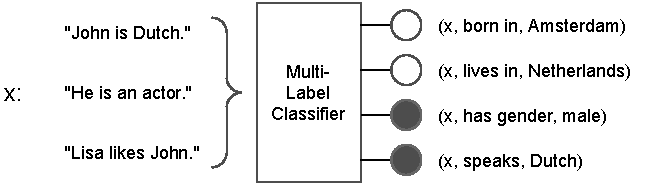
\includegraphics[width=\textwidth]{4_approach/1_texter/texter_idea}
    \caption{Basic concept behind the Texter: A multi-label classifier takes a query entity $x$'s texts and predicts common facts}
    \label{fig:4_approach/1_texter/texter_idea}
\end{figure}

A straight forward implementation of the described concept leads to the \emph{simple Texter}, which essentially consists of the embedding block presented in Section~\ref{subsec:4_approach/1_texter/1_text_embedding}, that embeds the input sentences, and the classification block introduced in Section~\ref{subsec:4_approach/1_texter/2_simple_model}, which produces the output logits. What the simple Texter is missing, is the desired prioritization between the entity's sentences. This feature is added by the more complex, \emph{attentive Texter} described in Section~\ref{subsec:4_approach/1_texter/3_attention_model}, which adds an attention mechanism between the embedding and classification blocks, that allows it to determine which sentence is most relevant for each class' prediction. That information is used in an attempt to improve the Texter's performance and returned as part of the prediction to provide the desired explanation to the user. Finally, Section~\ref{subsec:4_approach/1_texter/4_training} explains the training procedure. In Chapter~\ref{sec:5_experiments/4_texter}, both the simple and the attentive versions of the Texter are compared, whereby the simple Texter serves as a baseline to the attentive version.

\subsection{Text Encoding}
\label{subsec:4_approach/1_texter/1_text_embedding}
The first step of processing a query entity, which is the same for the simple and the attentive Texter, is embedding the entity's sentences in the embedding block. Thereby, each sentence is processed individually as illustrated in Figure~\ref{fig:4_approach/1_texter/1_text_embedding/embedding_block}: First, the sentence is split into words by the tokenizer, which are handled as integer IDs in further processing. Next, the words are embedded using some NLP approach, which could be a simple lookup table in the simplest case. As the last step, the word embeddings are combined to sentence embeddings in the embedding block's pooling layer.

\begin{figure}[t]
    \centering
    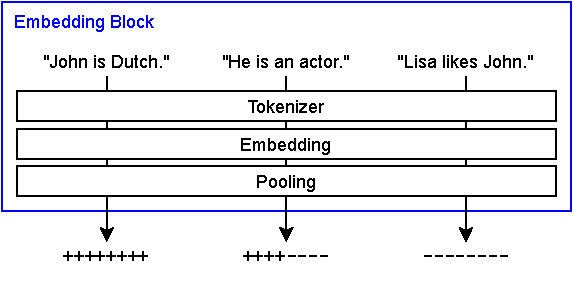
\includegraphics{4_approach/1_texter/1_text_embedding/embedding_block}
    \caption{The Texter's embedding block tokenizes sentences, embedds the tokens and combines the token embeddings to sentence embeddings in its pooling layer. Each sentence is processed individually. "+" and "-" denote positive and negative values in embedding vectors.}
    \label{fig:4_approach/1_texter/1_text_embedding/embedding_block}
\end{figure}

There are different possibilities for the concrete implementation of the individual parts, some of which will be examined in Chapter~\ref{ch:5_experiments}. In the final version of the Power model, a pre-trained transformer model is used for embedding the sentences' words, more precisely DistilBERT, a "distilled" variant of the transformer encoder BERT, reduced to the essentials~\cite{Sanh2019DistilBERTAD}. In contrast to a simple lookup table, DistilBERT is able to incorporate the context of a word into its embedding, which leads to more meaningful sentence embeddings. This choice of embedding approach also affects the tokenizer, the pooling layer, and even the input sentences: Thanks to context embedding, transformers can use special tokens that add additional information to the text. While a classical model cannot decide on the basis of the sentence "Lisa likes John." whether this sentence speaks for the class $(x, has~gender, male)$, a transformer is able to do so given the appropriately marked sentence "Lisa likes [START]John[END].". Especially for long, ambigious sentences performance can be increased significantly.

Beyond the input data, the use of a transformer also affects the tokenizer and the pooling layer. The tokenizer has to apply byte pair encoding (BPE) that is commonly used by pre-trained transformers, where sentences are not only divided into words, but words are further divided into subwords, thus keeping the vocabulary of the tokenizer small and allowing to exploit homorphisms between similar words. In addition, the tokenizer inserts the [CLS] and [SEP] introduced by BERT at the beginning and end of the sentence. That way, "Lisa likes [START]John[END]." becomes "[CLS]Lisa likes [START]John[END].[SEP]". While the [SEP] token is used to separate sentences and has no further meaning here, the embedding of the [CLS] token captures the meaning of the whole sentence and is therefore used as a sentence representation in the BERT paper~\cite{Devlin2019BERTPO}. However, the Power experiments have shown that performance can be increased if the word embeddings are also included, which is why the pooling layer of the embedding block averages all of a sentence's token embeddings, including the [CLS] embedding.


\subsection{Simple Model}
\label{subsec:4_approach/1_texter/2_simple_model}
During inference, the first step of processing a query entity, which is the same for both the simple and the attentive Texter, is embedding the entity's sentences in the embedding block. Thereby, each sentence is processed individually as illustrated in Figure~\ref{fig:4_approach/1_texter/1_simple_model/simple_architecture}: First, the sentence is split into words by the tokenizer, which are handled as integer IDs in further processing. Next, the words are embedded using some NLP approach, which could be a simple lookup table in the simplest case. As the last step in the embedding block, the word embeddings are combined to sentence embeddings in the pooling layer. The resulting sentence embeddings, that capture the sentences' overall meanings, are then passed on to the classification block where each of them is pushed through the neural multi-label classifier which consists of a single linear layer. Another pooling layer then combines the sentence-wise classification logits to the entity's logits. Finally, applying the sigmoid function to the entity's logits yields the class probabilites that state the probabilities of the associated facts about the query entity.

\begin{figure}[t]
    \centering
    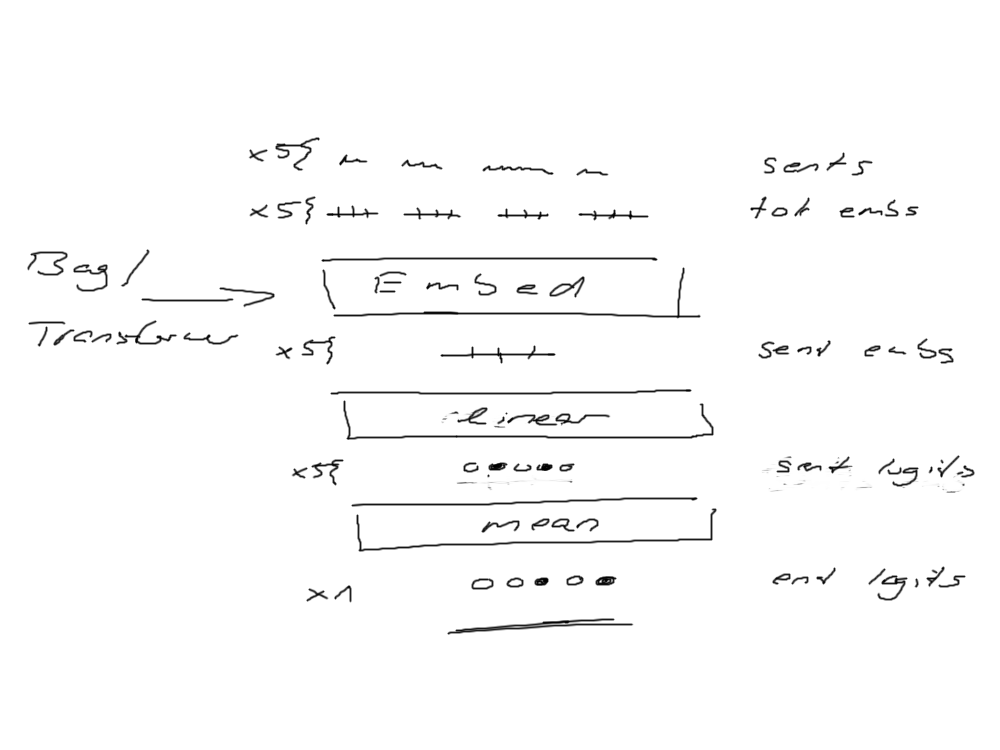
\includegraphics{4_approach/1_texter/1_simple_model/simple_architecture}
    \caption{Simple Texter Architecture; Each sentence is embedded and classified individually before the final pooling layer combines the results; "++++----" represents an embedding with positive and negative elements}
    \label{fig:4_approach/1_texter/1_simple_model/simple_architecture}
\end{figure}

Especially in the embedding block there are different possibilities for the concrete implementation of the individual parts to choose from, some of which will be examined in Chapter~\ref{ch:5_experiments}. In the final version of the power model, a transformer model is used for embedding the sentences' words, more precisely DistilBERT, a "distilled" variant of the transformer encoder BERT reduced to the essentials~\cite{Sanh2019DistilBERTAD}. In contrast to a simple lookup table, DistilBERT is able to incorporate the context of a word into its embedding, which leads to more meaningful sentence embeddings. This choice of embedding approach also affects the tokenizer, the pooling layer, and even the input sentences: Thanks to context embedding, transformers can use special tokens that add additional information to the text. While a classical model cannot decide on the basis of the sentence "Lisa likes John." whether this sentence speaks for the class $(x, has~gender, male)$, a transformer is able to do so given the appropriately marked sentence "Lisa likes [START]John[END].". Especially for long, ambigious sentences performance can be increased significantly.

Beyond the input data, the use of a transformer also affects the tokenizer and the pooling layer. The tokenizer has to apply byte pair encoding (BPE) that is commonly used by pre-trained transformers, where sentences are not only divided into words, but words are further divided into subwords, thus keeping the vocabulary of the tokenizer small and allowing to exploit homorphisms between similar words. In addition, the tokenizer inserts the [CLS] and [SEP] introduced by BERT at the beginning and end of the sentence. That way, "Lisa likes [START]John[END]." becomes "[CLS]Lisa likes [START]John[END].[SEP]". While the [SEP] token is used to separate sentences and has no further meaning here, the embedding of the [CLS] token captures the meaning of the whole sentence and is therefore  used as a sentence representation in the BERT paper~\cite{Devlin2019BERTPO}. However, the power experiments showed that performance can be increased if the word embeddings are also included, which is why the pooling layer of the embedding block averages all of a sentence's token embeddings, including the [CLS] embedding.

Less comprehensive processing steps happen in the classification block of the simple Texter: The sentence embeddings produced by the embedding block are pushed through the single linear classification layer whose multi-label output logits are averaged in the final pooling layer. The class probabilities calculated by applying the sigmoid function to the resulting entity logits are then used to sort the facts that have a probability greater than 50\%. Thus, the user of the model first receives the facts that are most likely to apply.


\subsection{Attention Model}
\label{subsec:4_approach/1_texter/3_attention_model}
While the simple Texter produces good evaluation results and does return a prioritized list of predicted facts, its prediction miss the desired explanation of why a fact is suggested. At this point, the attentive Texter extends the simple model by an attention mechanism that compares an entitiy's sentences to each other, forcing the model to favor sentences that are most relevant to the prediction of a certain fact. Besides the ability to provide an explanations for its predictions, the added attention mechanism should also increase the Texter's performance on datasets with multiple sentences per entity.

Technically, the attention mechanism is implemented as an attention block between the embedding and the classification blocks as shown in Figure~\ref{fig:4_approach/1_texter/2_attention_model/attention_architecture}. The embedding block is the same one used in the simple model, leveraging the DistilBERT encoder's contextual word embeddings to support marked input sentences and produce meaningful sentence embeddings. The classification block still produces the entity's multi-label output logits, but now uses multiple smaller linear layers to do so, due to the different outputs passed in from the attention block.

\begin{figure}[t]
    \centering
    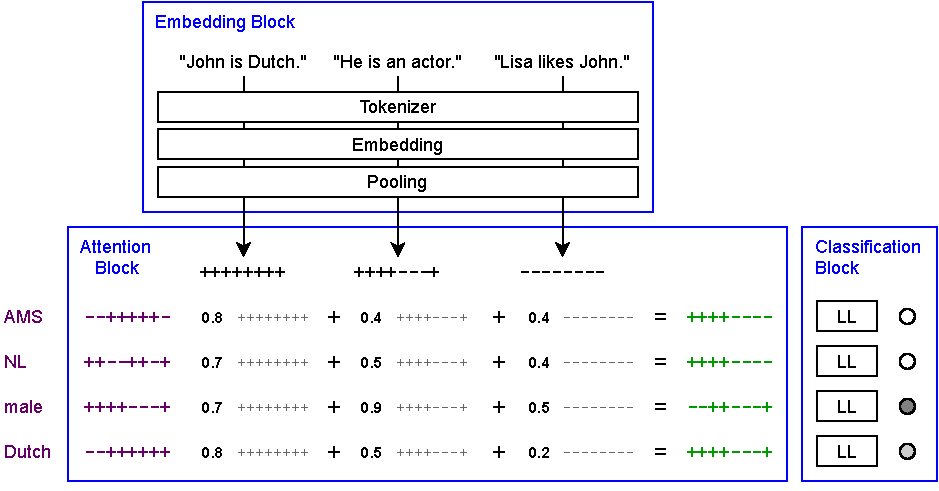
\includegraphics{4_approach/1_texter/2_attention_model/attention_architecture}
    \caption{Texter Architecture}
    \label{fig:4_approach/1_texter/2_attention_model/attention_architecture}
\end{figure}

The attention block now takes the sentence embeddings from the embedding block and compares them to so-called \emph{class embeddings} that represent each of the models output classes as a vector of the same dimension as the sentence embeddings. Given the set of input sentences $S$ and the set of classes $C$, the similarity between a class embedding $class_c$ and a sentence embedding $sent_s$ with $1 <= c <= |C|$ and $1 <= s <= |S|$ is calculated as the scalar product $\langle class_c, sent_s \rangle$ between the class and the sentece embedding. Given all class-sentence similarities for a certain class, the model can decide which sentence is matches the best for that class and deserves most attention when it comes to the decision whether the class holds true. Therefore, those similarity values are also referred to as attention values. To minimize the effect of sentences whose embeddings are very similar to a class embedding by pure chance, the attention values are furthermore normalized using the sigmoid function. Thus, the total attention matrix containing the attention values for all combinations of classes from $C$ and sentences from $S$ is calculated as shown in Equation~\ref{eq:4_approach/1_texter/2_attention_model/attention_matrix}.

\begin{align}
    A_{cs} = \sigma(\langle class_c , sent_s \rangle) && 1 <= c <= |C|, 1 <= s <= |S|
    \label{eq:4_approach/1_texter/2_attention_model/attention_matrix}
\end{align}

In the next step, the calculated attention values are used to combine the sentence embeddings to class-wise entity embeddings $ent_c$. As illstrated in Figure~\ref{fig:4_approach/1_texter/2_attention_model/attention_architecture} and formalized in Equation~\ref{eq:4_approach/1_texter/2_attention_model/ent_emb}, each sentence is thereby weighted by its class-wise attention value. The weighted sentences are then summed up to form class-wise entity embeddings whose purpose is to capture primarily those texts most relevant to the prediction of the respective class. Different from the simple Texter, the entity embeddings are then passed to the subsequent classification block instead of the original sentence embeddings.

\begin{align}
    ent_c = \sum_{s = 1}^{|S|} A_{cs} \cdot sent_s && 1 <= c <= |C|, 1 <= s <= |S|
    \label{eq:4_approach/1_texter/2_attention_model/ent_emb}
\end{align}

Similar to the simple Texter, the attentive Texter's classification consists of a $|C| \times d$ weight matrix and a bias vector of length $d$ where $d$ is the chosen embedding dimensionality for word, sentence, class and entity embeddings. In contrast to the simple model, however, given an entity embedding for a certain class, the weight matrix is not trained with respect to all output classes at once, but only with respect to the regarded class' ground truth output as illustrated in Figure~\ref{fig:4_approach/1_texter/2_attention_model/multi_linear}, which conceptually can be seen as training a separate single-output linear layer for each class and combining the outputs to the multi-label output thereafter. Formally, the models output classification outputs can be calculated as $out_c = \langle ent_c, W_c \rangle + b_c$ where $W_c$ and $b_c$ are the class' row in the weight matrix and its bias, respectively. The described approach to training the weight matrix was chosen, because a certain class' entity embedding focuses on the prediction of a single output class and would only hinder the learning process for other output classes it cannot make a qualified statement about.

\begin{figure}[t]
    \centering
    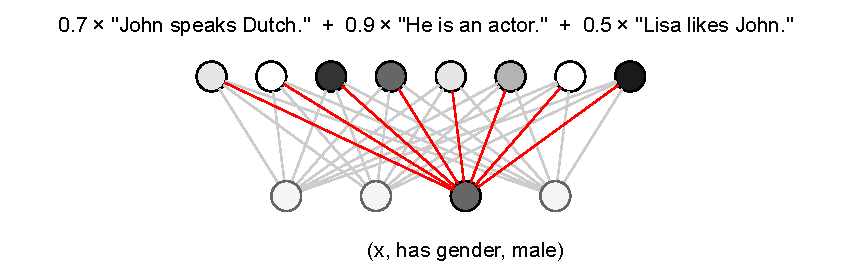
\includegraphics{4_approach/1_texter/2_attention_model/multi_linear}
    \caption{Multi-linear}
    \label{fig:4_approach/1_texter/2_attention_model/multi_linear}
\end{figure}

Similar to the simple Texter, following the core steps, the attentive Texter takes all classes whose confidences, that result from applying the sigmoid function to the output logits, is greater than 50\% to form their corresponding facts and sort them by confidence. In addition to the simple Texter, however, the attentive model provides the facts with the sentence weights as they result from the attention matrix in order to provide the user with an explanation for each fact's prediction. So, in the example, the fact $(John, has~gender, male)$, with a probability around 70\%, would be accompanied by the information that it was primarily suggested due to the sentence "He is an actor.", followed by "John speaks Dutch." and lastly "Lisa likes John.".

learnable class embs
sigmoid maps to (0, 1)
attention matrix A
total number of learnable params
in experiments: applied by an AdamW optimizer, a variant of the Adam optimizer that overcomes Adam's that keeps the training speed of Adam while keeping SGD's superior ability to generalize~, \cite{Loshchilov2019DecoupledWD}


\subsection{Training}
\label{subsec:4_approach/1_texter/4_training}
During supervised training, the Texter is fine-tuned to a specific dataset by repeatedly predicting facts, calculating its loss with regard to the ground truth class labels, and performing backpropagation to learn its randomly initialized parameters and fine-tune its word embeddings. The randomly initialized parameters include the classification block's weight matrix and bias vector, and, in case of the attentive Texter, also the attention block's class embeddings.

For the multi-label problem at hand, the binary cross-entropy (BCE) loss function is used. A convenient property of the BCE function is that it produces very large loss values for very wrong predictions which contributes to an initially fast learning process. To counteract unbalanced classes in the Texter dataset, the weighted binary cross entropy loss function (wBCE) shown in \autoref{eq:4_approach/1_texter/4_training/wbce} is used. It calculates the loss for the multi-label output logits $x$ and the respective ground truth labels $y$, both of which are c-dimensional vectors with $c$ being the number of output classes. Without the weights, the model would learn that it gets off best by always making negative predictions for very rare classes. This would be good for high accuracy, but is bad for the metrics used during evaluation, which do not measure true negatives. A class' weight $w_c$ is calculated as the reciprocal of the class' frequency it occurs in the training data with. A class that is true for every fifth entity, for example, would be assigned a class weight of five. To make the logits comparable with the usual 0 and 1 ground truth labels, they are normalized to range $[0, 1]$ by applying the sigmoid function.

\begin{align}
    wBCE(x, y) = - \frac{1}{C} \sum_{c = 1}^C w_c \cdot log(\sigma(x)) + (1 - y) \cdot log(1 - \sigma(x))
    \label{eq:4_approach/1_texter/4_training/wbce}
\end{align}

Besides the loss function, another important aspect of training is the way the gradients calculated from the loss are applied during backpropagation, i.e. the way to perform gradient descent. Plain batch gradient descent is generally too slow and while stochastic gradient descent and mini-batch gradient descent improve in this matter, they still cannot be considered fast. While many projects use the adaptive Adam optimizer, popular for its speed, this work uses the AdamW optimizer, recommended for the finetuning of transformers~\cite{Loshchilov2019DecoupledWD}. According to its inventors, it keeps the speed of Adam, while approaching the generalization capabilities of SGD with momentum.

